%!TEX root = ../thesis.tex
\newchap{Signal reconstruction and interpretation}\label{sec:kin}
\vspace{-1cm}
\minitoc
\vspace{0.5cm}
This chapter is dedicated to the kinematical reconstruction and interpretation of the signal events.
\\
\\
First, a straightforward unidimensional feature ranking is presented to show which are the observables that characterize the signal events and that distinguish them from the main source of background, and then the jet-parton assignment problem on signal events is tackled.
\\
\\
Initially, we tackle the jet-parton assignment in a simplified form by focusing on the selection of the jet associated with the b quark parton that arises in the decay of the top quark that decays into the leptonic W boson. This simplified benchmark is used to perform a feature ranking exploiting the $N+1,\: N-1$ method and to select the best model that will be employed in the complete jet-parton assignment task and that will be adapted to discriminate the signal from the background, as presented in the next chapter.
\\
\\
All the investigations presented in this chapter are carried out within the Muon signal region, as defined in Table \ref{tab:event_selection}, after the kinematic reconstruction of the neutrino described in sec. \ADDREF.\\
\begin{minipage}[H]{\linewidth}
\begin{minipage}{0.35\linewidth}
        \centering
        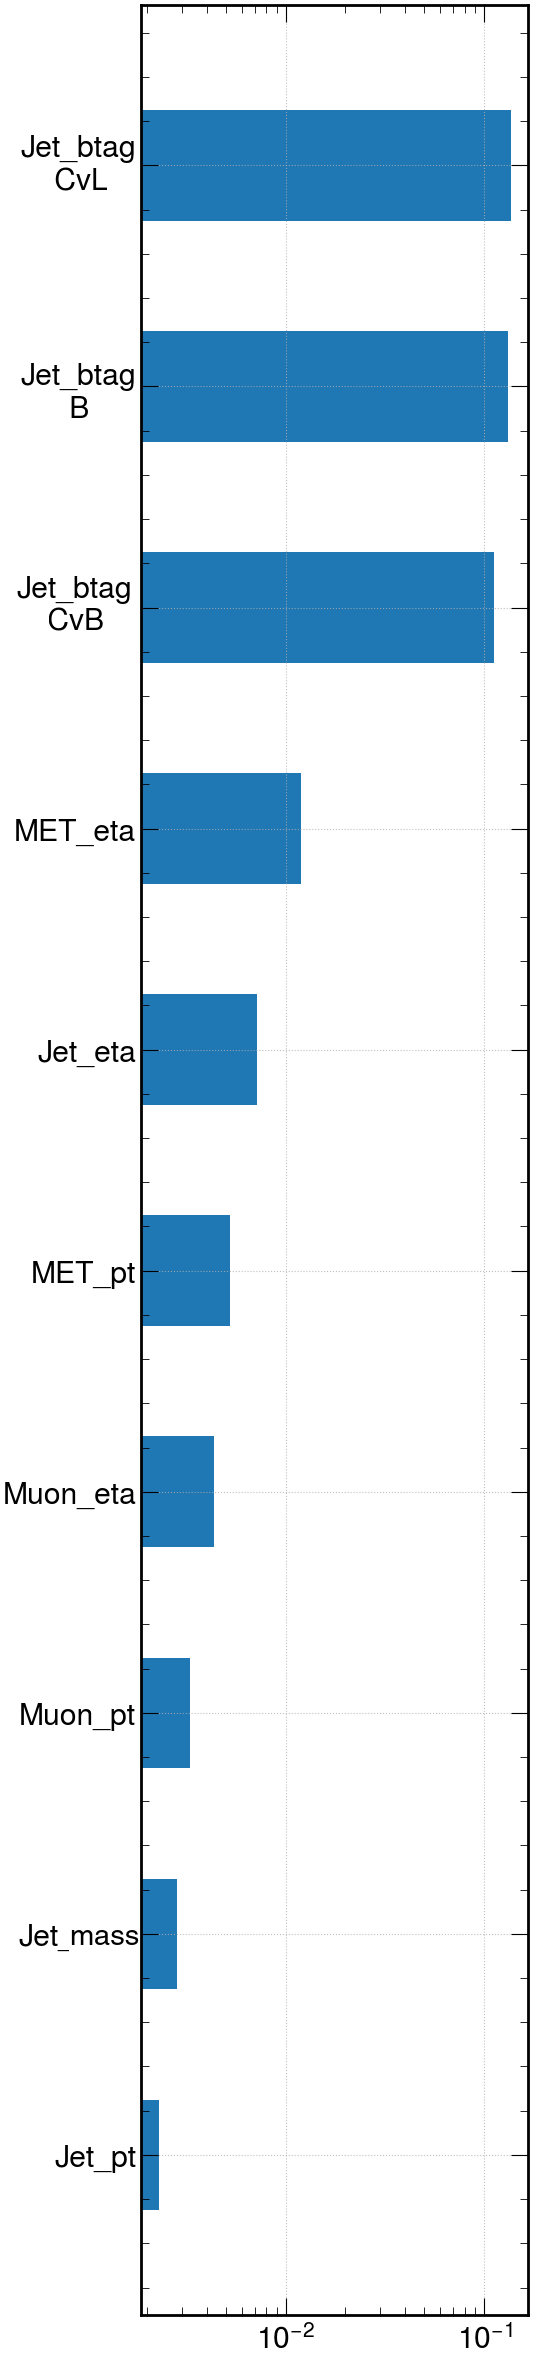
\includegraphics[height=0.92\textheight]{fig//chap08-kin_reco/ranking1D.png}
        \captionof{figure}{Unidimensional feature ranking using the metric $d$ between flattened signal observables and \ttbar semileptonic observables }
        \label{fig:1Drank}
\end{minipage}
\hfill
\begin{minipage}{0.62\linewidth}
\section{Unidimensional feature ranking}
The most straightforward approach for identifying discriminative features that separate the signal from the background is to examine the distributions of various observables and select those with the most distinct shapes.\\
The "shape difference" between two histograms can be quantified by the following metric

\begin{equation}
    d=\frac{1}{2}\sum_b \bigg| y_b^{(1)}-y_b^{(2)} \bigg|
\end{equation}
where $y_b^{(i)}$ is the bin height of the b-th bin of the i-th histogram. The histograms are normalized such that their integral is 1.\\
\\
The metric $d$ is computed between the signal and the $\ttbar$ semileptonic process, which is the primary source of background.\\
All observables are flattened, \ie all objects in the events are pooled together in the same histograms, neglecting the event's structure.\\
\\
The ranking is performed in the Muon channel, after the preselection.\\\\
The outcome of the unidimensional ranking is shown in \Fig{fig:1Drank} and, without any surprise, the observables with the highest ranking are the ones related to the b-tagging with $d\sim 0.1$, while Other observables yield results that are an order of magnitude smaller, and the latest are due mostly to statistical fluctuations.\\
\\
However, this method is not satisfactory since it does not account for correlations between the observables. Therefore, more sophisticated multivariate methods, such as neural networks, will be employed. \\\\\\\\\\    
\end{minipage}
\end{minipage}
\section{Jet-parton assignment}
The Jet-Parton assignment (JPA) task consists of associating a jet to each of the four quark partons that belong to the signal final state to reconstruct the event's topology and kinematics.\\
\\
This task is challenging due to the combinatorial nature: if there are N jets in an event, there are a total of $N!/(N-4)!$ possible combinations for assigning a jet to the 4 partons, so, for example, in the case of an event with 10 jets, there are over 5000 possible combinations.\\
\\
Typically, the assignment is accomplished through a kinematic fit that consists of finding the combination of jets for each event that minimizes the chi-square of all the invariant masses.
\begin{equation}
    \chi^2=\frac{(m_{j_1j_2}^{\text{inv.}}-m_W)^2}{\Gamma^2_W}+\frac{(m_{j_1j_2j_3}^{\text{inv.}}-m_t)^2}{\Gamma^2_t}+\frac{(m_{j_4\ell\nu}^{\text{inv.}}-m_t)^2}{\Gamma^2_t}
\end{equation}
where $\Gamma_\PW$ and $\Gamma_t$ are the experimental dijet and trijet invariant mass resolution widths of the W and top quark hadronic decays, respectively.\\
This is an unsupervised approach but in this work, another approach is employed, leveraging supervised multivariate models like neural networks that allow us to exploit not only the kinematic variables of jets but also their flavor score and the correlations between all the observables.


\begin{minipage}{\linewidth}
    \begin{minipage}{0.35\linewidth}
        \begin{table}[H]
            \centering
            \begin{tabular}{c|c}
            \toprule
                \multicolumn{2}{c}{\textbf{Signal events}}\\
                \multicolumn{2}{c}{\textbf{Muon region}}\\
                \multicolumn{2}{c}{$5.7 \cdot 10^7$}\\
                \midrule
                \multicolumn{2}{c}{$\bm{\Delta R(\textbf{part.-jet})<0.4}$}\\
                \multicolumn{2}{c}{$\forall \textbf{partons}$}\\
                \multicolumn{2}{c}{$2.5 \cdot 10^7$}\\
                \midrule
                 \textbf{Training} & \textbf{Validation}\\
                 $2.0 \cdot 10^7$& $5\cdot 10^6$\\
                 \bottomrule
            \end{tabular}
            \caption{Composition of the training and validation datasets employed to perform the JPA.}
            \label{tab:dataset}
        \end{table}
    \end{minipage}
    \hfill
    \begin{minipage}{0.6\linewidth}
    The dataset employed to conduct this study is composed of $5.7 \cdot 10^7$ signal events that have passed the muon channel selections.\\
    In order to avoid ambiguities and to assign to each jet a label, a further requirement is imposed: all the four quark partons at the generator level in the event have to match a distinct reconstructed jet through the condition $\Delta R<0.4$.\\
    The fraction of signal events in the muon channel that satisfy this requirement is $43\%$. Of these 25 million of events, $80\%$ are used to train the models, while the remaining $20\%$ are reserved for the model validation.       
    \end{minipage}
\end{minipage}

\subsection{Leptonic bJet benchmark}
In principle, the b quark parton in the signal final state originating by the leptonic top decay is the easiest to assign to a reconstructed jet for two reasons:
\begin{itemize}
    \item The top quarks are produced back-to-back and the decay products of each top quark are boosted along the the respective top quark momentum direction.\\
    Given that, the b parton originating by the leptonic top decay is closer on average to the lepton in the $\phi-\eta$ plane than the other quark partons.
    \item Since it is a heavy flavor parton, we can exploit the b-tagging capabilities of the experiment. In an ideal situation, the b-tagging would simplify the problem by reducing the number of jet candidates to just three.
\end{itemize}
Several multivariate models were evaluated to select the most accurate that will be used to perform the jet-parton assignment on all four quark partons.\\
\\
In the upcoming sections, we will refer to the b parton originating by the leptonic top decay as "the leptonic b parton" and the corresponding jet with "the leptonic b jet".\\
As well, the problem of assigning the leptonic b parton to a jet for each event will be denoted as "simplified JPA problem".
\subsubsection*{Jet-wise models}
The initial class of models tested uses only observables associated with the jets as input.\\
In other words, the event's structure is disregarded and the data provided to the models is a matrix that has different jets on the rows and different features of the jets on the columns.  

\begin{minipage}{\linewidth}
\begin{minipage}{0.4\linewidth}
The inputs fed to the models are shown in Tab. \ref{tab:jet_inputs}.\\
\\
The simplified jet-wise JPA problem is a binary classification task where the model's goal is to determine whether a particular jet is associated with the leptonic b parton.\\
\\
The event's structure is reconstructed afterward, and the jet with the highest score within each event will be classified as the leptonic b jet, and the accuracy is defined as the ratio between the number of events in which the leptonic b parton is associated with the right jet and the total number of events.
\\
\\

    
\end{minipage}
\hfill
\begin{minipage}{0.55\linewidth}
\begin{table}[H]
 \fontsize{10pt}{10pt}\selectfont
 \centering
\begin{tabular}{l|l}
\toprule
\textbf{Input feature} & \textbf{Description} \\
\midrule
Jet\_pt & Jet $p_T$ \\
\midrule
Jet\_eta & Jet $\eta$\\
\midrule
Jet\_btag & \DeepJet b-tag score \\
\midrule
Jet\_CvL. & \DeepJet CvL score\\
\midrule
Jet\_CvB &  \DeepJet CvB score\\
\midrule
\multirow{2}{*}{Jet\_mass} & Invariant mass of the\\
&weighted sum of Jet's constituents. \\
\midrule
\multirow{2}{*}{max\_dEta\_Jets}& $\max(\Delta \eta)$ computed with\\
&respect to other jets in the event. \\
\midrule
\multirow{2}{*}{min\_dEta\_Jets} & $\min(\Delta \eta)$ computed with\\
&respect to other jets in the event. \\
\midrule
\multirow{2}{*}{max\_dPhi\_Jets} & $\max(\Delta \phi)$ computed with\\
&respect to other jets in the event. \\
\midrule
\multirow{2}{*}{min\_dPhi\_Jets} & $\min(\Delta \phi)$ computed with\\
&respect to other jets in the event. \\
\midrule

dPhi\_Jet\_nu & $\Delta \phi$ Jet-$\nu$\\
\midrule
dEta\_Jet\_nu & $\Delta \eta$ Jet-$\nu$\\
\midrule
dEta\_Jet\_mu & $\Delta \eta$ Jet-$\mu$\\
\midrule
dPhi\_Jet\_mu & $\Delta \phi$ Jet-$\mu$ \\
\midrule
T\_mass &  Jet$+\mu+\nu$ invariant mass\\
\bottomrule
\end{tabular}
\caption{Input features of the jet-wise models tested for the simplified JPA task.\\}
\label{tab:jet_inputs}
\end{table}
\end{minipage} 
\end{minipage}

The jet-wise models tested are three: 
\begin{itemize}
    \item \textbf{Fisher discriminant} The Fisher's linear discriminant \ADDREF is a simple model whose goal is to find a hyperplane that maximizes the separation between the classes maximizing the between-class variance and minimizes the within-class variance.\\
    \\
    The fisher discriminant identifies two regions, separating the predicted leptonic b jets from the other jets. The absolute value of the score assigned to each jet is the distance between the jet represented in the jet's feature space and the separating hyperplane, while the score sign will be positive if the jet belongs to the predicted leptonic b jet region, and negative otherwise.
    \\
    \\
    This is a linear model and its complexity is not sufficient to tackle the JPA problem. Indeed, its accuracy on both training and validation datasets is just $45\%$.
    \item \textbf{k-nn}
    \item \textbf{MLP}
\end{itemize}



\subsubsection*{{$N-1,N+1$} ranking}
\subsection{JPANet}
\subsection{Full Jet-parton assignment}

